\pagebreak
\hypertarget{GuardarFinalizar}{\section{Guardar y/o Finalizar}}

Al llenar todos los datos correctamente, el Docente dará click en el botón:

\begin{figure}[H]
    \centering
    
\includegraphics[width=0.1\linewidth]{images/SP6/BotonFinalizar.jpeg}
    \caption{Botón Finalizar} 
\end{figure}

Se mostrara la siguiente pantalla:

\begin{figure}[H]
    \centering
    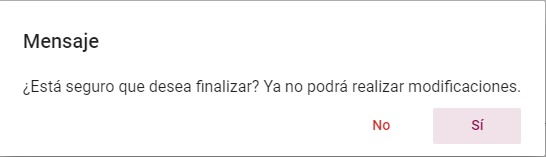
\includegraphics[width=0.6\linewidth]{images/SP6/DeseaRegistro.jpeg}
    \caption{¿Seguro que desea finalizar el registro?} 
\end{figure}

Al dar clic en \IUbutton{Aceptar} y si no se presentan errores se muestra el mensaje:


\begin{figure}[H]
    \centering
    
\includegraphics[width=0.4\linewidth]{images/SP6/MSGFINALIZAR.jpeg}
    \caption{Registro exitoso}
    \label{mensaje5}
\end{figure}

El sistema bloquea el formulario y se procede al siguiente formulario. 


Para continuar con el registro, usted tendrá que  dar click en \IUbutton{Cancelar}, el mensaje se cerrara y usted continuara 
en el formulario para terminar el registro.

Si el usuario requiere guardar el avance que ha ingresado: 

\begin{figure}[H]
    \centering
    
\includegraphics[width=0.1\linewidth]{images/SP6/BotonGuardar.jpeg}
    \caption{Botón Guardar} 
\end{figure}

El sistema guarda la información ingresada y muestra el mensaje: 

\begin{figure}[H]
    \centering
    
\includegraphics[width=0.4\linewidth]{images/SP6/MSGGUARDAR.jpeg}
    \caption{Botón Avances Guardados exitosamente.} 
\end{figure}
\pagebreak


